\documentclass[10pt,a4paper]{article}
\usepackage[margin=1.65 cm,top=1.4 cm,bottom=1.5 cm]{geometry}
\usepackage[T1]{fontenc}
\usepackage[utf8]{inputenc}
\usepackage{lmodern,microtype,booktabs,tabularx,array,amsmath,graphicx,xcolor,hyperref,enumitem,fancyhdr}
\definecolor{navy}{HTML}{183B56}\definecolor{teal}{HTML}{187F80}
\hypersetup{colorlinks=true,urlcolor=teal,linkcolor=navy,pdftitle={Thesis Progress Update: Routing Cost and Training-Energy Payback},pdfauthor={Eren Olmez}}
\setlength{\parindent}{0 pt}\setlength{\parskip}{4 pt}\setlength{\emergencystretch}{2 em}
\renewcommand{\arraystretch}{1.12}
\setlist[itemize]{leftmargin=1.2 em,itemsep=1 pt,topsep=2 pt}
\pagestyle{fancy}\fancyhf{}\fancyhead[L]{\small\color{navy}Energy-efficient input-based model routing}
\fancyhead[R]{\small 29 October 2026}\fancyfoot[C]{\small\thepage}\setlength{\headheight}{13 pt}
\newcommand{\heading}[1]{\section*{\color{navy}#1}}
\newcommand{\smallcap}[1]{{\footnotesize\color{navy}#1}\par}
\begin{document}
\begin{center}
{\Large\bfseries\color{navy}Thesis Progress Update}\\[3 pt]
{Eren Olmez}\\{29 October 2026}
\end{center}\vspace{-8 pt}
\heading{1. Meeting questions and results across batch sizes}
The meeting requested batch-level accuracy, latency and energy statistics including batch 1, clearer plots, and the number of deployment inferences needed to recover router-training energy. This update joins the saved 13 October correctness results and 20 October controls with the new batch 1 investigations. No larger-batch experiments were rerun.

\textbf{What is being routed?} The router is a small predictor that chooses which classifier will process an input. Our correctness TinyCNN predicts each candidate's probability of success; a calibrated cost rule selects one classifier, which predicts the CIFAR-100 class. For a batch, probabilities are averaged to select one model for all its images. Fitting used 3,000 images and calibration 2,000; evaluation uses all 10,000 balanced test images (100 per class).

\textbf{Three distinct questions.} Study A changes the \emph{router architecture}; Study B changes \emph{how the same TinyCNN system loads and executes classifiers}. Separate engineering probes test ideas not adopted in those full routing runs. More training and per-image batching are investigated separately on page 4. These are not one system containing every optimization.

\textbf{Baseline and pass.} Eligible static means one fixed classifier selected on calibration data to meet the accuracy allowance, without routing. Savings compare fresh measurements in the same execution mode (eager or Graph). An accuracy pass alone does not imply an efficiency win.

\textbf{Comparison rule.} Below, fix the \emph{latency objective and 1-percentage-point accuracy allowance}, and retain all three seeds 42/45/48. Historical costs are five-repeat medians per seed; new batch 1 costs are one full sweep per seed. A pass requires accuracy $\geq 84.80\%$, relative to fresh ResNet-101 FP32's 85.80\%. Low cost alone is not success.
\begin{center}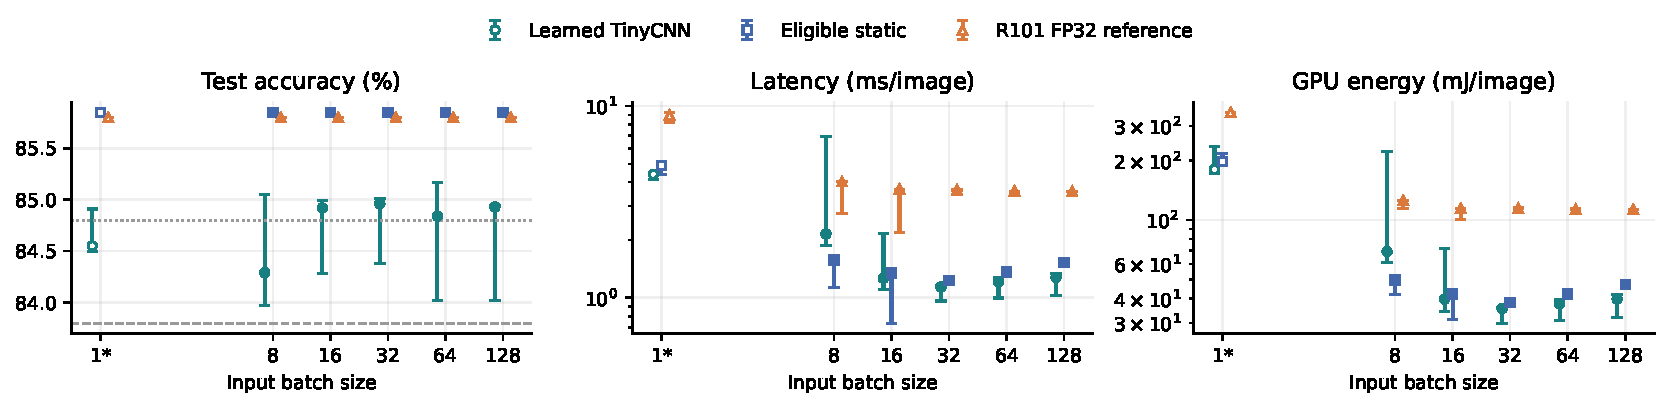
\includegraphics[width=\linewidth]{images/batch_comparison.pdf}\end{center}\vspace{-8 pt}
\smallcap{Dots are medians across three seeds; vertical ranges show the seed minimum/maximum, not confidence intervals. Open markers at batch 1 are deliberately not connected to the historical series. Latency/energy include preprocessing, routing, dispatch and classification; startup is separate.}
\begin{center}\small\begin{tabular}{@{}llrrrr@{}}
\toprule
Batch & Protocol & Accuracy (\%) & ms/batch & GPU mJ/batch & Pass\\
\midrule
1 & 6 resident & 84.50--84.91 & 4.15--4.46 & 171.4--235.4 & 1/3\\
8 & 213 choices, cache 2 & 83.97--85.05 & 15.04--55.57 & 485.5--1772.0 & 1/3\\
16 & 213 choices, cache 2 & 84.28--84.99 & 17.58--34.48 & 549.8--1144.0 & 2/3\\
32 & 213 choices, cache 2 & 84.38--85.01 & 30.74--36.88 & 961.3--1151.4 & 2/3\\
64 & 213 choices, cache 2 & 84.02--85.17 & 63.55--80.79 & 1981.5--2511.5 & 2/3\\
128 & 213 choices, cache 2 & 84.02--84.94 & 130.78--169.97 & 4052.9--5306.1 & 2/3\\
\bottomrule
\end{tabular}\end{center}
\smallcap{Batch 1 here is Study A's resident-eager TinyCNN control, not Study B's graph-optimized variant. Table costs average executed batches, including the batch 128 tail (79 batches per 10,000 images). Historical 213 choices/two-engine cache versus new 6 resident candidates are different protocols, not a controlled scaling experiment.}

\textbf{Earlier evidence, retained.} Across all 120 historical settings (both objectives and four allowances), 53 passed accuracy; 31 of these saved latency and 31 saved GPU energy versus their eligible static comparator. The 20 October uniform-random controls reached only 36.26\% accuracy at batch 64 and 36.25\% at 128, versus learned ranges 81.86--85.64\% and 82.25--85.39\%. Beating this weak control does not establish a win over a strong static classifier. Fixed 80\%-pruned controls reached only 0.93--22.55\%: their low costs came with unacceptable accuracy.

\newpage
\heading{2. Batch 1: smaller routers versus runtime optimization}
\textbf{Study A: change the router, keep classifier execution fixed.} Four compact CPU routers and the existing GPU TinyCNN each processed all 10,000 test images for three seeds, once per seed. All six classifiers, execution contexts and buffers stayed loaded in GPU memory, so warm inference had no loading/eviction misses. Standard eager execution was used, without CUDA Graphs.
\begin{center}\small\begin{tabular}{@{}lrrrrrr@{}}
\toprule
Router & Accuracy (\%) & ms/image & GPU mJ/image & Pass 1 pp & Pass 2 pp & Device\\
\midrule
Depth 3 tree & 83.89--85.02 & 4.12--4.98 & 174.5--227.0 & 2/3 & 3/3 & CPU\\
Logistic & 84.01--84.62 & 5.43--5.89 & 221.1--291.3 & 0/3 & 3/3 & CPU\\
Thumbnail MLP & 84.27--84.98 & 4.45--5.16 & 171.6--220.8 & 1/3 & 3/3 & CPU\\
Boosted depth 2 & 84.19--85.01 & 6.59--7.64 & 246.7--305.4 & 1/3 & 3/3 & CPU\\
TinyCNN control & 84.50--84.91 & 4.15--4.46 & 171.4--235.4 & 1/3 & 3/3 & GPU\\
Eligible static & 85.85--85.85 & 4.37--5.10 & 191.6--217.4 & 3/3 & 3/3 & --\\
\bottomrule
\end{tabular}\end{center}
\smallcap{Ranges across the three seeds. Pass counts the 1 pp accuracy gate; latency is total warm wall time, not neural-router time alone. The four compact alternatives run on the CPU; reported GPU energy excludes their CPU consumption. The static alternative is validation-selected, not selected from test results.}

\textbf{Study A result.} The depth 3 tree was promising but no method passed accuracy while saving both latency and GPU energy versus eligible static. Seed 42 tree: 84.87\%, 5.59\% lower latency but 4.41\% more GPU energy. Seed 45: 85.02\%, 3.49\% less GPU energy but 1.82\% slower. Smaller predictors were not automatically cheaper overall.

\textbf{Study B: implement loading/switching optimizations in full TinyCNN runs.} These were \emph{not just microbenchmarks}: the same original TinyCNN weights and six-classifier pool were tested in five runtime variants. Three seeds, three repeats, five routed modes and four matched static controls gave 81 full 10,000-image sweeps. These optimizations were not all applied to every compact CPU router. Study A/B ran in separate sessions; compare each with its own controls, not as a paired speedup.
\begin{center}\small\begin{tabularx}{\linewidth}{@{}Xrrrc@{}}
\toprule
TinyCNN runtime mode & ms/image & GPU mJ/image & Pass & Selection\\
\midrule
Engine files, capacity 2 & 15.91--23.15 & 528.9--806.3 & 1/3 & Dynamic\\
RAM bytes + reuse, capacity 2 & 7.61--8.20 & 243.8--285.0 & 1/3 & Dynamic\\
Six resident, eager & 6.66--7.73 & 197.0--351.6 & 1/3 & Dynamic\\
Six resident, CUDA Graphs & 6.07--6.42 & 190.1--215.3 & 1/3 & Dynamic\\
RAM + switching-aware, capacity 2 & 6.02--6.94 & 207.4--222.1 & 3/3 & Constant\\
\bottomrule
\end{tabularx}\end{center}
\smallcap{Each entry summarizes three-repeat medians across all three seeds (range); Pass counts seeds meeting 1 pp. Warm inference includes routing, selection, loads, evictions and classification; initial setup is separate. RAM-byte caching avoids repeated disk reads, not GPU deserialization. Resident modes eliminate warm misses. CUDA Graphs replay captured GPU work to reduce launch overhead.}

\textbf{What helped?} Host-byte caching plus reuse/less cleanup reduced recorded latency from 15.91--23.15 to 7.61--8.20 ms/image while preserving each seed's selections; this is a combined change, not an isolated attribution. Six-model residency removed loading misses. Resident Graph routing's seed 42 case passed accuracy (84.91\%) and recorded 9.07\% latency/4.20\% GPU-energy savings versus \emph{graph-enabled eligible static}. Other seeds failed accuracy. Even seed 42's repeat-level latency savings ranged$-2.40$ to$+25.01\%$: this is not a consistent win on every repeat.

\textbf{What did not establish dynamic benefit?} Switching-aware calibration charged measured miss costs, but all three policies then chose R101 FP16 for every image. Avoiding switches helped execution, yet this is effectively static selection. Static timings varied substantially; lower cost relative to an expensive loading implementation is not necessarily a win over eligible static.

\textbf{Separate engineering probes, not deployed in Studies A/B.}
\begin{itemize}
\item \emph{GPU selection:} compute scores/argmax on GPU and read only the model ID; the CPU still launches a separate classifier engine. Controlled selector timings overlapped (CPU 4.352, Torch GPU 4.368, TensorRT FP32 4.390 ms/image). No reliable speedup; FP32 changed 15/105 near-tie choices.
\item \emph{Native GPU conditional prototype:} two classifiers were combined so only the selected branch ran. It passed branch/parity checks, but took 4.123 ms/image versus 3.955 ms CPU dispatch. This was validation-only engineering, not a full accuracy-qualified routing policy.
\item \emph{Batch 1-specific engine profiles:} a dedicated R34 INT8 build changed 40/100 probe classes (68.06\% validation versus 73.84\% original). It remains quarantined, not counted as an accuracy-preserving optimization. A separate residency probe found 53/12/18 safe models depending on loading order, not an absolute hardware maximum.
\end{itemize}

\newpage
\heading{3. Router-training energy and inference break-even}
\textbf{Measured missing numerator.} Three 20-epoch correctness-router fits were repeated under GPU energy monitoring using seeds 42/45/48. This measures the fitting recipe, not the historical runs retrospectively.
\begin{center}\small
\begin{tabular}{@{}lrrr@{}}\toprule
Router seed & GPU fit energy (J) & Fit-window time (s) & Epochs\\\midrule
42&270.437&11.138&20\\45&201.185&8.389&20\\48&195.008&8.266&20\\\bottomrule
\end{tabular}
\end{center}
Median fit energy is 201.185 J (range 195.008--270.437 J). The measurement includes initialization, fitting and epoch-checkpoint writes. It excludes supervision generation, policy calibration, TensorRT export, final weight writing and CPU/whole-PC energy. A deployed seed is charged its own fitting cost, \emph{not the sum of all three exploratory fits}.

\textbf{Correct denominator: the saving on every inference.} Let $E_{\mathrm{fit}}$ be that router's GPU fitting joules, $e_{\mathrm{static}}$ the comparator's GPU J/image and $e_{\mathrm{route}}$ the \emph{complete routed system's} GPU J/image:
\[
N_{\mathrm{payback}}=\left\lceil\frac{E_{\mathrm{fit}}}{e_{\mathrm{static}}-e_{\mathrm{route}}}\right\rceil .
\]
There is \textbf{no valid payback} when the denominator is nonpositive or held-out accuracy fails. For full batches, the corresponding count is
$\lceil E_{\mathrm{fit}}/[B(e_{\mathrm{static}}-e_{\mathrm{route}})]\rceil$.
This accounts for routing overhead; dividing training energy by static inference energy alone would be incorrect.

\textbf{Worked measured example (historical batch 64, energy objective, seed 48,1 pp).} Accuracy is 85.18\%, so the allowance passes. Eligible static uses 0.0607284 J/image and routing uses 0.0403774 J/image. Saving is 0.0203510 J/image; with 195.008 J of fit energy, repayment is 9,583 images.

\begin{center}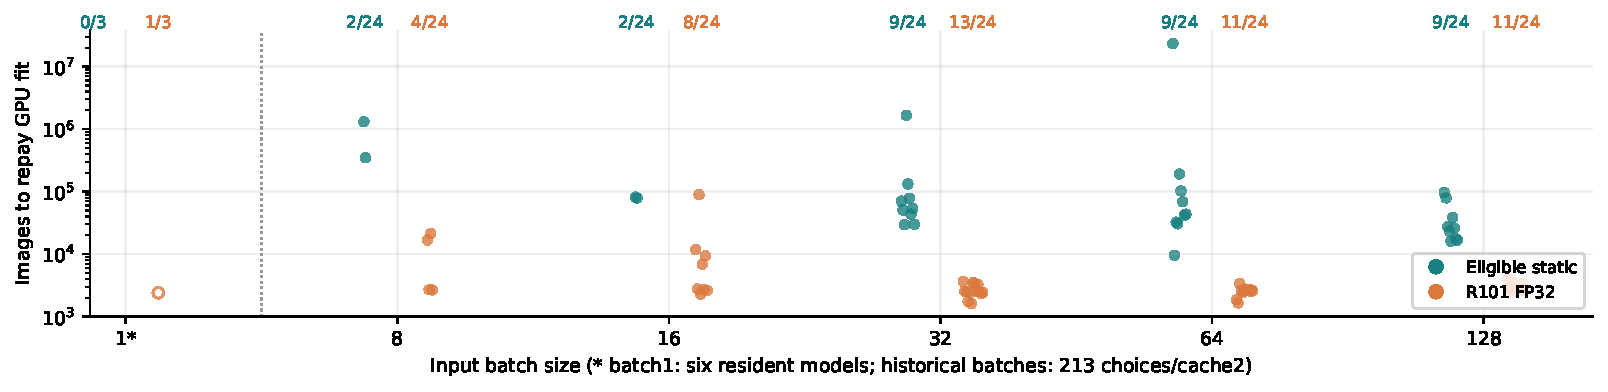
\includegraphics[width=\linewidth]{images/payback_comparison.pdf}\end{center}\vspace{-7 pt}
\smallcap{Batch 1* is \textbf{Study A only}: three TinyCNN seeds, latency/1 pp, six resident classifiers with eager execution. It is not the graph-optimized Study B. Historical batches retain 24 settings each. Dots require accuracy compliance and positive energy saving; counts show valid/available cases. Open marker: seed 42 only. Blue: eligible static; orange: R101 FP32.}
\begin{center}\small\begin{tabular}{@{}rll ll@{}}
\toprule
& \multicolumn{2}{c}{Compared with eligible static} & \multicolumn{2}{c}{Compared with R101 FP32}\\
\cmidrule(lr){2-3}\cmidrule(l){4-5}
Batch & Settings repaying & Images before repayment & Settings repaying & Images before repayment\\
\midrule
1* & No payback & \textemdash & 1 of 3 & 2,399\\
8 & 2 of 24 & 350,497--1,314,076 & 4 of 24 & 2,670--21,288\\
16 & 2 of 24 & 79,015--81,556 & 8 of 24 & 2,279--89,265\\
32 & 9 of 24 & 29,522--1,672,462 & 13 of 24 & 1,614--3,659\\
64 & 9 of 24 & 9,583--23,494,940 & 11 of 24 & 1,653--3,382\\
128 & 9 of 24 & 16,089--96,831 & 11 of 24 & 2,571--3,970\\
\bottomrule
\end{tabular}\end{center}
\textbf{Batch 1 example (Study A, seed 42).} Fitting uses 270.437 J; routed energy is 0.2353969 J/image versus 0.3481643 J/image for R101 FP32: $\lceil 270.437/(0.3481643-0.2353969)\rceil=2,399$ images. Eligible static uses only 0.2173951 J/image, so routing cannot repay energy against it. Other seeds fail the original accuracy gate. CPU-router fit energy is unmeasured, so no CPU-router payback is claimed.


\textbf{Optimized Study B is a different case.} Seed 42 resident-Graph routing uses 0.2153288 GPU J/image and passes accuracy; repayment is 28,621 images versus graph-enabled eligible static. Do not compare this directly with Study A\textquotesingle s 2,399 images versus FP32: the runtime, baseline and measurement session differ.


\textbf{Limits.} These are GPU-fit-only estimates combining separate training and inference sessions, not whole-PC lifetime-energy accounts. Tiny positive savings create huge, unstable break-even values. Hardware/session variation and the omission of supervision, calibration and export prevent a precise full-pipeline payback claim.

\newpage
\heading{4. Can training changes or per-image choices improve routing?}
This section changes the learned predictor or decision granularity, \emph{not loading/switching optimizations}. It is separate from Study B: supervision variants used the six-resident eager runtime; the batch 8 experiment measured grouping overhead explicitly.

\textbf{Data quantity, training and calibration.} A predefined seed 42 screen compared 1,000/2,000/3,000 fitting images at 20 epochs and unweighted/balanced 60-epoch alternatives selected on 600 internal tuning images. The reserved 2,000 calibration images were not used for training; policies used 500/1,000/2,000-image subsets. All five new routers passed TensorRT parity before 20 full test sweeps with the original CNN and fresh controls.
\begin{center}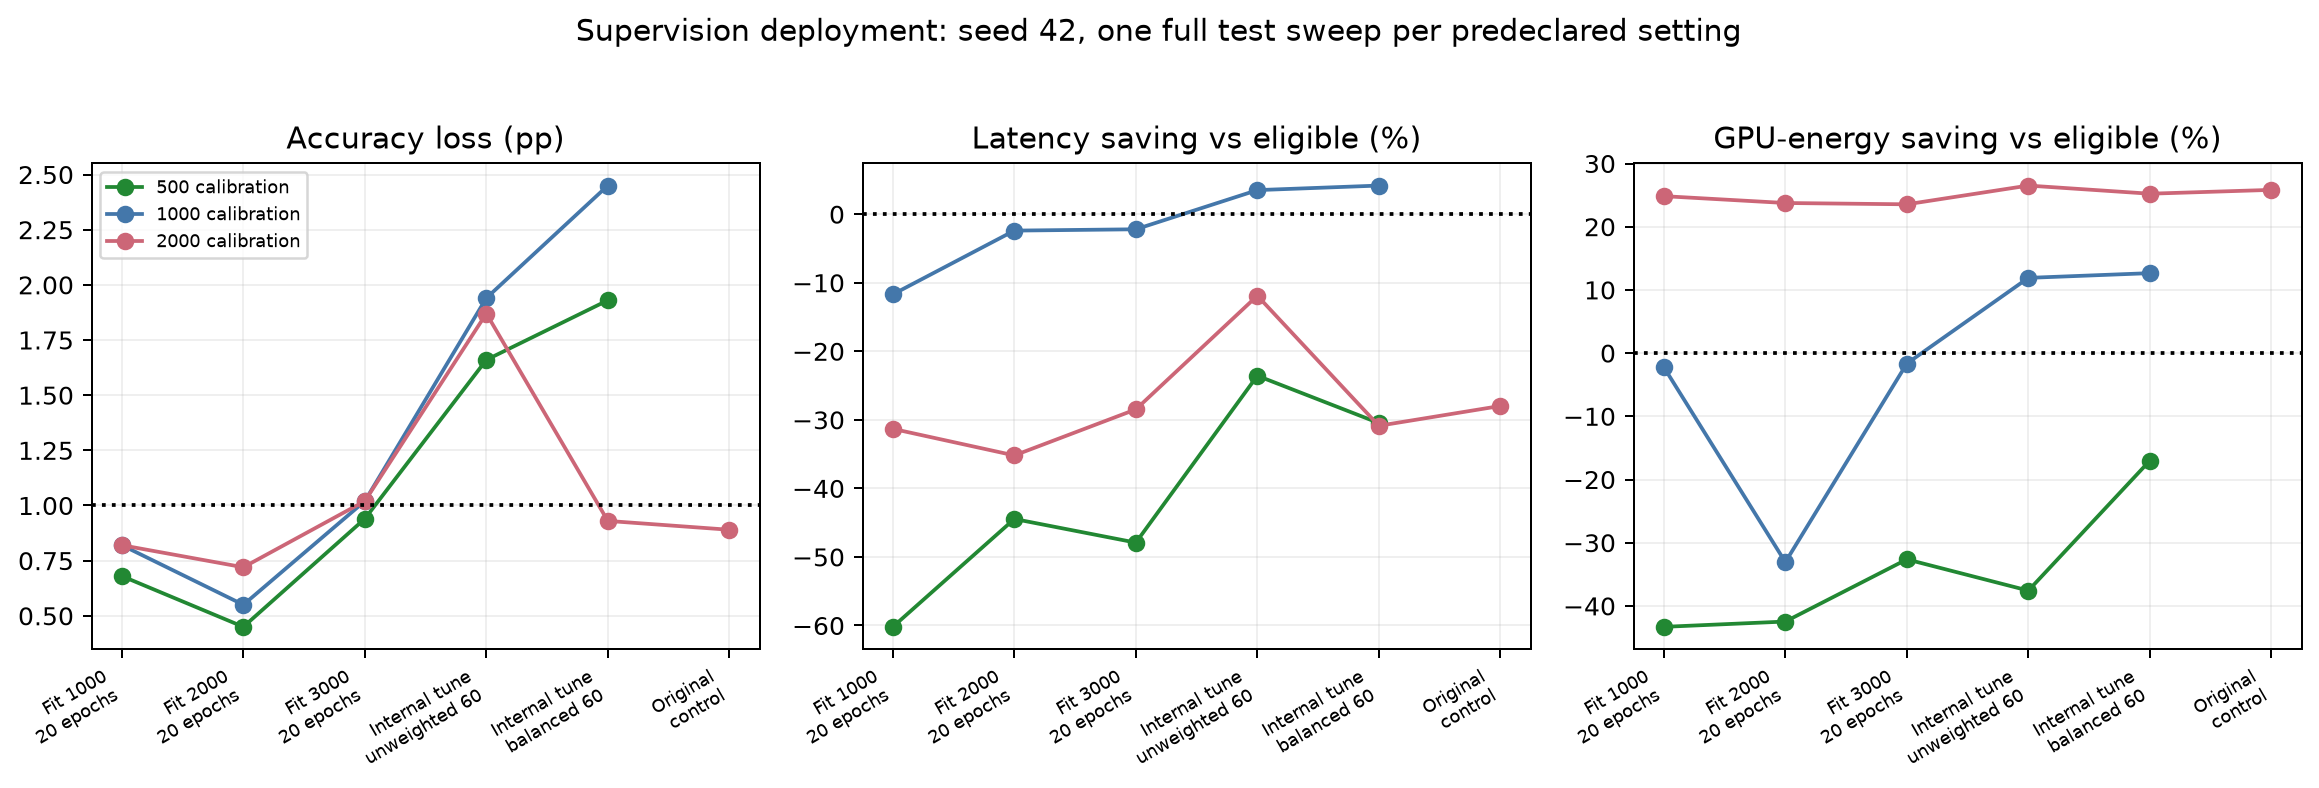
\includegraphics[width=\linewidth]{images/supervision_deployment.png}\end{center}\vspace{-6 pt}
\smallcap{Seed 42, one repeat per predeclared setting; all negative and failed cases remain. The 1 pp accuracy gate is shown at left. Latency/GPU-energy savings at right use the fresh static control matching each calibration subset. No model or calibration size was chosen retrospectively from test performance.}
\textbf{Finding.} Nine of 16 routed cases passed accuracy; none also saved both latency and GPU energy versus eligible static. Four passed accuracy and saved GPU energy, giving fit-only payback despite worse latency. More data or longer training did not consistently improve deployment; this single-seed screen does not establish a best recipe.

\textbf{One model per batch versus per-image specialists.} The three original routers produced eight separate 213-output vectors. Batch 8 images were grouped by selected classifier, inferred and scattered back into order. All gather/group/scatter/dispatch costs and final CPU class output were timed.
\begin{center}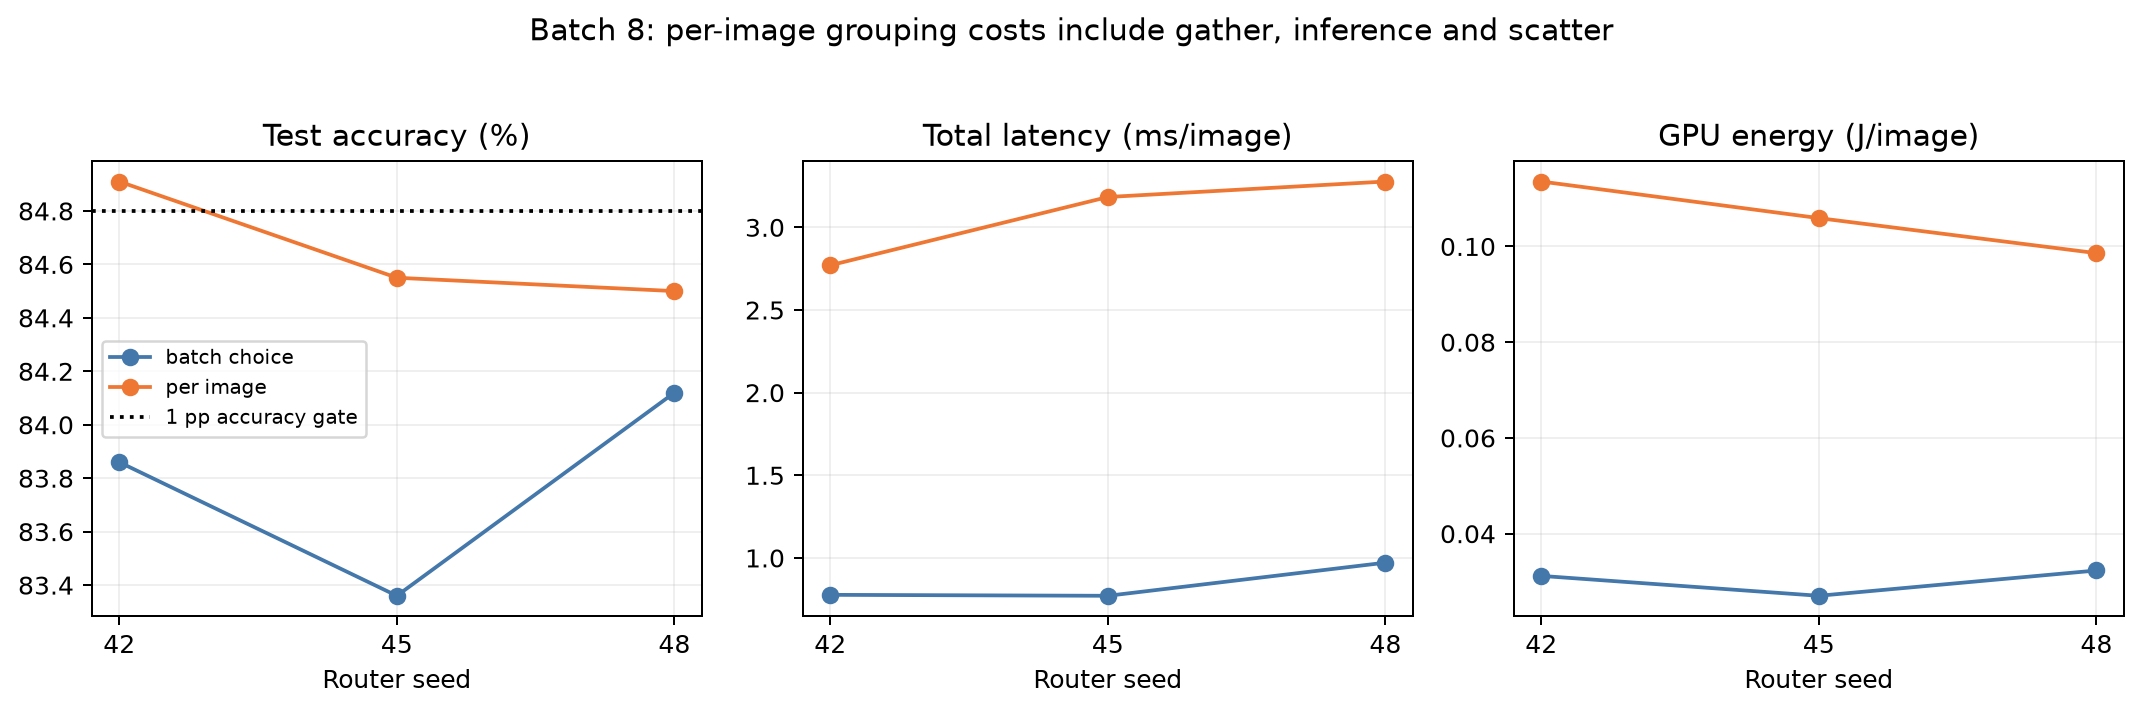
\includegraphics[width=\linewidth]{images/batch8_grouping.png}\end{center}\vspace{-6 pt}
\smallcap{Three seeds, three repeats and fresh static controls: 36 full sweeps. This is a separate 6-resident-model experiment, not a direct rerun of the 13 October 213-choice batch 8 rows.}
Per-image accuracy was 84.91/84.55/84.50\%; only seed 42 passed 1 pp. It required 2,570/2,659/2,801 classifier invocations versus 1,250 for one choice per batch, and 2.77--3.28 ms/image versus 0.77--0.97. Better specialization did not compensate for execution overhead in this implementation.

\smallcap{\textbf{Evidence and reproducibility.} Saved 13 October correctness results and 20 October uniform/80\%-pruned controls; new audited summaries dated 28--29 October. \texttt{report\_data.json} records source hashes and exact values; \texttt{build\_report\_assets.py} generates tables and plots without running inference.}
\end{document}
